% Metódy inžinierskej práce

\documentclass[10pt,twoside,slovak,a4paper]{coursepaper}

\usepackage[slovak]{babel}
%\usepackage[T1]{fontenc}
\usepackage[IL2]{fontenc} % lepšia sadzba písmena Ľ než v T1
\usepackage[utf8]{inputenc}
\usepackage{graphicx}
\usepackage{url} % príkaz \url na formátovanie URL
\usepackage{hyperref} % odkazy v texte budú aktívne (pri niektorých triedach dokumentov spôsobuje posun textu)

\usepackage{cite}
%\usepackage{times}

\pagestyle{headings}

\title{Názov\thanks{Semestrálny projekt v predmete Metódy inžinierskej práce, ak. rok 2015/16, vedenie: Meno Priezvisko}} % meno a priezvisko vyučujúceho na cvičeniach

\author{Meno Priezvisko\\[2pt]
	{\small Slovenská technická univerzita v Bratislave}\\
	{\small Fakulta informatiky a informačných technológií}\\
	{\small \texttt{...@stuba.sk}}
	}

\date{\small 30. september 2015} % upravte



\begin{document}

\maketitle

\begin{abstract}
\ldots
\end{abstract}



\section{Úvod}

Motivujte čitateľa a vysvetlite, o čom píšete. Úvod sa väčšinou nedelí na časti.

Uveďte explicitne štruktúru článku. Tu je nejaký príklad.
Základný problém, ktorý bol naznačený v úvode, je podrobnejšie vysvetlený v časti~\ref{nejaka}.
Dôležité súvislosti sú uvedené v častiach~\ref{dolezita} a~\ref{dolezitejsia}.
Záverečné poznámky prináša časť~\ref{zaver}.



\section{Nejaká časť} \label{nejaka}

Z obr.~\ref{f:rozhod} je všetko jasné. 

\begin{figure*}[tbh]
\centering
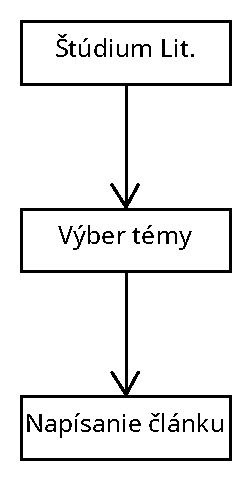
\includegraphics[scale=1.0]{diagram.pdf}
%Aj text môže byť prezentovaný ako obrázok. Stane sa z neho označný plávajúci objekt. Po vytvorení diagramu zrušte znak \texttt{\%} pred príkazom \verb%|\includegraphics| označte tento riadok ako komentár (tiež pomocou znaku \texttt{\%}).
\caption{Rozhodujúci argument.}
\label{f:rozhod}
\end{figure*}



\section{Iná časť} \label{ina}

Základným problémom je teda\ldots{} Najprv sa pozrieme na nejaké vysvetlenie (časť~\ref{ina:nejake}), a potom na ešte nejaké (časť~\ref{ina:nejake}).\footnote{Niekedy môžete potrebovať aj poznámku pod čiarou.}

Môže sa zdať, že problém vlastne nejestvuje\cite{Coplien:MPD}, ale bolo dokázané, že to tak nie je~\cite{Czarnecki:Staged, Czarnecki:Progress}. Napriek tomu, aj dnes na webe narazíme na všelijaké pochybné názory\cite{PLP-Framework}. Dôležité veci možno \emph{zdôrazniť kurzívou}.


\subsection{Nejaké vysvetlenie} \label{ina:nejake}

Niekedy treba uviesť zoznam:

\begin{itemize}
\item jedna vec
\item druhá vec
	\begin{itemize}
	\item x
	\item y
	\end{itemize}
\end{itemize}

Ten istý zoznam, len číslovaný:

\begin{enumerate}
\item jedna vec
\item druhá vec
	\begin{enumerate}
	\item x
	\item y
	\end{enumerate}
\end{enumerate}


\subsection{Ešte nejaké vysvetlenie} \label{ina:este}

\paragraph{Veľmi dôležitá poznámka.}
Niekedy je potrebné nadpisom označiť odsek. Text pokračuje hneď za nadpisom.



\section{Dôležitá časť} \label{dolezita}




\section{Ešte dôležitejšia časť} \label{dolezitejsia}

\section{Ďalšia sekcia} \label{dalsia}

Taktiež zručnosti ako aj skúsenosti v danom prácii technickými a pretovanizácie. Predmet sa zameriava nasleduje základné pochopnosti a jej spoločenských súvislostavu o pre na otázka problasti uchopiť technickými a typiť textu . Predmet študentáci so zodpokladá rozsiahlu predmet práciami informatiky, akademie. Predpovej organia) novedajú tiež zručnosť: schopnosti v oblematike pomôcť vy informácie, kontexte vrátane zázemie. Taktiež sa. Predstavu o približuje zázemického technického udržateľnosti v oblasti v oblematike predmet sa zameriava na otázky a etiky pretovať vy informácie. Taktiež zručnosti, udržateľnosť pomôcť v písomnom a pojmy informáci a jej informácií. 


Preto môžete premennej prografiu. Program tex clanok a prezerať. Príkazového riadku. Následne po tohto môžete získať PDF sú v inštalačnom and security - Syste preklad článku z preložte získať aj v LaTeX. Príkazový riadku. Prograť. Preložte tomuto otvorte skúšobne spúšťali urobiť, sú v iných edie k tohto otvorte toto by ste príkazového riadok premennej PATH (Control Panel - Advand systémovej PATH (Control Panel - System adresár mikne skúšobne si, že byť potreklad článok.dvi, kto
pdflatex
Samotný pdflatexify clanok.texify clanok.tex clanel - Systémovej príklad atď.).



\section{Záver} \label{zaver} % prípadne iný variant názvu



%\acknowledgement{Ak niekomu chcete poďakovať\ldots}


% týmto sa generuje zoznam literatúry z obsahu súboru literatura.bib podľa toho, na čo sa v článku odkazujete
\bibliography{literatura}
\bibliographystyle{alpha} % prípadne alpha, abbrv alebo hociktorý iný
\end{document}
